\section{Результаты}
\label{sec:conclusion-future}
В рамках этой работы была реализована стадия компиляции, направленная на деление структур по типам, с целью их последующей векторизации.
Было показано, что это помогает распределению структур на векторные регистры и уменьшает количество обращений в память.
Разработан алгоритм с делением структур неограниченной вложенности.
Реализация внедрена в графический компилятор Intel.
Предложен способ замены инструкций с сохранением корректности работы программы.

Для тестирования алгоритма использовались приложения из открытого стека рендеринга Intel (OSPray, Embree).
Была оценена корректность алгоритма (прошли все тесты) и его положительное влияние на производительность скомпилированной программы.

\begin{figure}[ht]
    \centering
    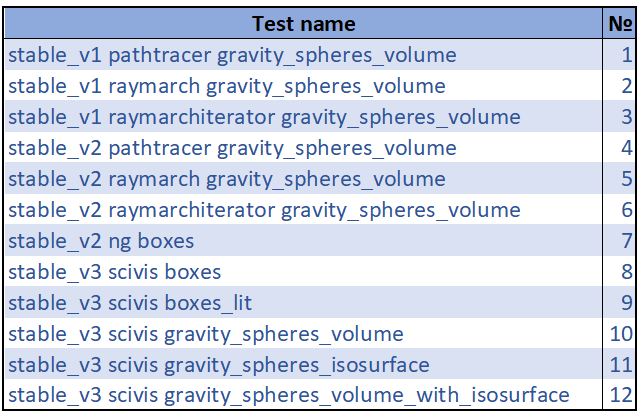
\includegraphics[scale=0.55]{Images/results_name.png}
    \caption{Названия тестов.}
    \label{fig:results_name}
\end{figure}

\begin{figure}[ht]
    \centering
    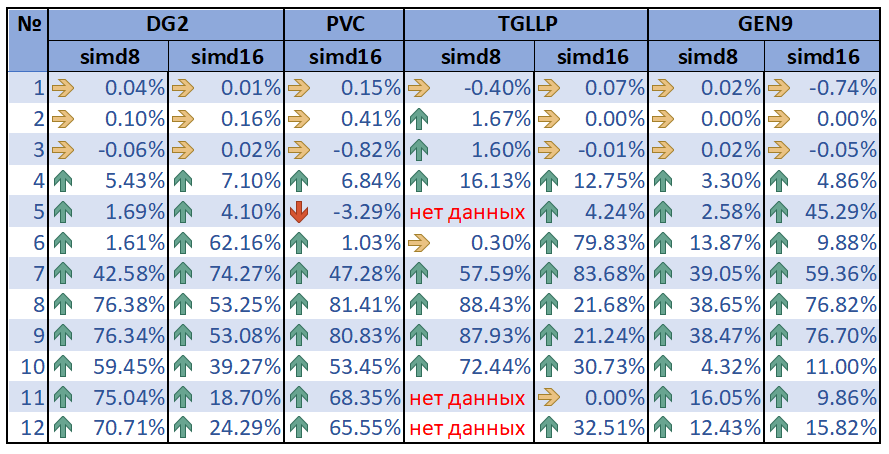
\includegraphics[scale=0.54]{Images/results_pure.png}
    \caption{Результаты работы.}
    \label{fig:results_pure}
\end{figure}

На рис.~\ref{fig:results_name} и рис.~\ref{fig:results_pure} показан прирост скорости работы приложений при различной ширине SIMD и на различных платформах.
В тех тестах, где структуры не были использованы, нет прироста производительности.
Однако с ростом сложности программ и с увеличением случаев обращения к структурам данных наблюдается прирост производительности вплоть до 88\%.

Разработанная оптимизация открывает целый спектр дальнейших возможных улучшений, включая разбиение массивов и векторов структур, введение пользовательских эвристик, поддержку указателей и многое другое.